Unter dem Begriff "Backend" versteht man Komponenten eines digitalen Systems, die den Betrieb des Programms ermöglichen und vom Benutzer nicht ersichtlich sind. ...[TODO]
\newline
Eine Backend-Anwendung kann direkt mit dem Frontend interagieren und dessen Benutzerdienste unterstützen sowie die Schnittstellen mit allen erforderlichen Ressourcen anbieten.

\subsection{Datenbank}
Hier steht mein BackendDatenbank Text.

\subsubsection{Einrichtung}
Hier steht mein Imlementierung Text.

Die Serverzuständigkeiten lassen sich in folgende Aspekte zusammenfassen:
\begin{itemize}
\item Empfangen und Beantworten der Clientanfragen
\item Routing der Anfragen zu den entsprechenden Abhandlungsroutinen
\item Überprüfen der Identität des Clients
\item Kommunikation zur Datenbank für die persistente Speicherung der Zustände der Nutzer und ihrer Präferenzen, Swipes und Matches.
\item Matching-Algorithmus
\end{itemize} 

In den folgenden Unterkapitel wird auf die Einrichtung des Node.js-Webservers und der MongoDB-Datenbank, auf die Erstellung der sicheren Kommunikationsschnittstelle und auf die Implementierung der serverzuständigen Funktionalitäten eingegangen.

\subsection{Webserver}
Hier steht mein BackendServer Text.

\subsubsection{Einrichtung}
Zunächst...


\subsubsection{Sicherheit}
Den Server gilt es zu schützen.

\subsubsection{Webserver}
Den Server gilt es zu schützen.



\subsection{Firebase}
\label{sec:implementierung_firebase}
Firebase bietet viele verschiedene Werkzeuge zur Entwicklung und Überwachung von Mobil- und Webanwendungen.
Nach dem Konzept nach Kapitel \ref{sec:concept} beschränkt sich der Aufgabenbereich des Firebase Backends auf Nutzerauthentifizierung, Verwaltung der Nutzerdaten und der Chatfunktion.
Die hierfür genutzten Werkzeuge werden im Folgenden besprochen.\\
Grundlegend muss zunächst eine Anwendung erstellt, ein Firebase Projekt aufgesetzt und diese zusammen verknüpft werden.
Sobald dieser Prozess abgeschlossen ist, muss sichergestellt sein, dass Firebase in der Anwendung initialisiert wird.

\subsubsection{Authentifizierung}
Um Nutzern eine sichere Registrierung, bzw. An- und Abmeldung ermöglichen zu können bietet Firebase das Authentifizierungswerkzeug. 
Dieser Backendservice verfügt über unterschiedliche Authentifizierungsmethoden.
Um es zu nutzen, muss nur die jeweilige Methode ausgewählt werden. \\

\noindent
In unserem Fall wurde die E-Mail und Passwort Authentifizierung gewählt, um unabhängig von Drittanbietern zu sein.
Nun muss das SDK \texttt{firebase\_auth} integriert werden und mithilfe der Funktionen \texttt{createUserWithEmailAndPassword()} bzw. \texttt{signInWithEmailAndPassword()} ein Nutzer registriert und angemeldet werden.
Hierbei können mithilfe von Fehlercodes geeignete Fehlermeldungen erstellt werden. 
Zusätzlich besitzt die Klasse \texttt{User} das Feld \texttt{emailVerified} (Boolean) und die Methode \texttt{sendEmailVerification()}, wodurch eine Verifizierung der E-Mail über Nachrichtenvorlage durchgeführt wird.
Ist ein Nutzer einmal authentifiziert, muss unterschieden werden, welchen Bildschirm er sehen darf.
Hierzu wird darauf geachtet, ob ein aktueller Nutzerobjekt existiert.
Ist dies nicht der Fall, wird der Anmeldebildschirm angezeigt; ansonsten der Hauptbildschirm.
\medspace
\begin{lstlisting}[caption= Anzeige abhängig ob ein aktueller Nutzer existiert]
	// Globale Instanz des Authentifizierungsservice
	final AuthService auth = Provider.of(context).auth;
	return FutureBuilder<User>(
		future: auth.getCurrentUser(),
		builder: (BuildContext context, AsyncSnapshot<User> snapshot) {
			// Existiert ein Nutzer, wird der Hauptbildschirm angezeigt
			if (snapshot.hasData) {
				return MessageHandler();
			} 
			// Zeige ansonsten den Login-Bildschirm
			else {
				return SignUpScreen(authFormType: AuthFormType.signIn);
			}
		}
	);
\end{lstlisting}
\medspace

\subsubsection{Nutzerdaten}
Bei der Authentifizierung eines Nutzers wird mittels des Auth-Services ein Nutzerobjekt erstellt.
Dieses kann folgende Felder besitzen:
\begin{itemize}
	\item Einzigartige Identifikation (UID)
	\item E-Mail Adresse
	\item Namen
	\item Bild-URL
\end{itemize}
Es ist jedoch nicht möglich über diesen Service weitere Eigenschaften abzuspeichern.
Diese müssen über zusätzliche Speicherwerkzeuge, wie beispielsweise Cloud Firestore (siehe \ref{sec:firestore}) gesichert werden.\\
\\
Hierzu wurde die Sammlung \enquote{users} erstellt und bei der Registrierung für jeden Nutzer ein Dokument mit der selben ID, wie die Nutzer UID erstellt. 
Dadurch ist sichergestellt, dass es ein einzigartiges Dokument und der Zugriff einfach geregelt ist.
Hier werden nun weitere Eigenschaften gesichert, welche teilweise ausschließlich zu Anzeigezwecken in Firebase doppelt abgespeichert werden.
\begin{itemize}
	\item Anzeigename
	\item E-Mail
	\item Wohnort, welcher aus den wichtigsten Städten Deutschlands bestehen
	\item Geschlechter, nach welchen gesucht wird
	\item Eigenes Geschlecht
	\item Lieblingsfilm
\end{itemize}
Unser Nutzer jedoch speichert seine Profil und Hintergrundbilder weder im Auth-Service Nutzerobjekt noch im Cloud Firestore Dokument.
Bei Auth-Service lässt sich lediglich die URL zu einem einzigen Bild hinterlegen.
Bei Firestore ist es zwar möglich eine theoretisch unbegrenzte Menge an Bild URLs abzuspeichern, jedoch muss der Nutzer die Möglichkeit haben seine eigenen Bilder hochzuladen und nicht nur eine URL auf ein bereits hochgeladenes Bild abspeichern.\\
\\
Hierfür bietet Firestore das Werkzeug Storage. 
Wie in Kapitel \ref{sec:firebase_storage} beschrieben, können hier Nutzerinhalte hoch- und heruntergeladen werden. 
Dazu wird beim ersten Hochladen ein Ordner für jeden Nutzer erstellt.
Darin werden daraufhin die Bilder unter dem Namen \texttt{profile-picture} oder \texttt{background-picture} jeweils abgespeichert und eventuell überschrieben.
Mit einer Funktion kann über einen Boolean-Parameter entschieden werden, welches Bild somit angezeigt wird.
\medspace
\begin{lstlisting}
	Future<String> getPictureFromStorage(String uid, bool isProfilePicture) async {
		try {
			// Die Referenz auf Storage
			Reference storage = FirebaseStorage.instance.ref();
			// Ordner UID mit Datei profile-picture oder background-picture
			Reference ref = storage.child(uid)
				.child(isProfilePicture ? '/profile-picture' : '/background-picture');
			// Gebe die URL zum Download zurueck
			return await ref.getDownloadURL();
		} on Exception catch (e) {
			// Fehlerbehandlung eine Ebene oberhalb
			throw e;
		}
	}
\end{lstlisting}
\medspace
\subsubsection{Chatfunktion}
Damit Nutzer bei einem erfolgreichen Match sich unterhalten und vielleicht auch verabreden können, muss eine Anwendung dieser Art eine Chatfunktion bieten.
Diese Funktion jedoch beschränkt sich auf eine 1-zu-1 Kommunikation, es werden also keine Gruppenchats benötigt.
Aus welchem Grund wird hierfür jedoch Firebase verwendet?\\

\noindent
Da Google weltweit über Server verfügt, ist diese Chatanwendung mithilfe von Firebase direkt auch global verfügbar.
Zudem würde der Backend Server, welcher die Filmdaten bereitstellt und Nutzer über Matching Algorithmen zusammenführt, zusätzlich durch Netzwerkverkehr der Chatanwendung belastet.
Hierfür bietet Firebase extra auf Skalierung ausgelegte Werkzeuge, damit sich Entwickler nicht zwingend mit diesen Problematiken auseinandersetzen müssen.
Zusätzlich müsste mit einem separaten Server die Sicherheit und Wartung behandelt werden; dies wird bei Firebase direkt gemacht.
Ein großer Nachteil ist jedoch, dass mit Firebase die Ende-zu-Ende Verschlüsselung nicht direkt gegeben ist und nachträglich eigenhändig oder über externe Bibliotheken eingefügt werden muss (weiterführende Informationen in Kapitel \ref{sec:firebase_security}).
Bei einem separaten Server ist dies zwar ebenfalls nicht gegeben, aber kann über das Design des Features im Voraus geregelt werden.\\
\\
\noindent
Grundsätzlich benötigt man für die Chaträume eine Sammlung in Firebase, welche die beteiligten Nutzer beinhaltet. 
Ein Dokument dieser Sammlung bekommt eine einzigartige ID bestehend aus den jeweiligen UIDs der Nutzer, die durch  einen Unterstrich zusammengefügt sind.
Damit diese ID wirklich einzigartig ist und nicht zwei Chaträume mit den IDs \enquote{Nutzer1\_Nutzer2} und \enquote{Nutzer2\_Nutzer1} entstehen können, werden bei der Erstellung beide UIDs alphabetisch verglichen und entsprechend angeordnet (siehe Code \ref{lst:chat_uid_sorting}).\\

\begin{lstlisting}[caption=Sortierung der UIDs, label=lst:chat_uid_sorting]
	// Vergleicht die Strings, setzt den im Alphabet vorher kommenden zuerst
	if (firstUID.compareTo(secondUID) <= 0)
		roomID = firstUID + "_" + secondUID;
	else
		roomID = secondUID + "_" + firstUID;
\end{lstlisting}

In diesem Dokument werden nicht nur die UIDs der einzelnen Nutzer abgespeichert, sondern aus Anzeigegründen auch die Nutzernamen und die Raum-Identifikation selbst.
Zusätzlich benötigt dieser Raum auch eine Möglichkeit Nachrichten abzuspeichern.
Hierzu existiert eine Untersammlung \texttt{messages}, in welcher einzelne Nachrichten als Dokumente gespeichert werden.
Diese wiederum beinhalten den eigentlichen Nachrichtentext, die UID des Senders, die des Empfängers und einen Zeitstempel.
Die UIDs werden einerseits dazu benötigt, um in der Oberfläche die Nachricht links- oder rechtsbündig anzuzeigen (siehe Abbildung \ref{fig:chat_e}).
Andererseits werden sie für die Benachrichtigungen benötigt, also welcher Nutzer auf seinem Gerät eine Benachrichtigung erhalten soll.\\
\\
Für die Benachrichtigungen wird das Werkzeug Cloud Functions verwendet.
Es bietet die Aus"-füh"-rung von serverseitigem Code unter bestimmten Bedingungen.
Um eine solche Funktion nun ausführen zu können, muss eine weitere Sammlung \texttt{unreadMessages} existieren.
In diese wird beim Versenden einer Nachricht das selbe Nachrichtendokument wie in der Untersammlung \texttt{messages} gespeichert.
Dieser Schreibvorgang löst nun die Funktion von Cloud Functions aus, welche eine Benachrichtigung zusammenbaut (siehe Code \ref{lst:chat_functions}).
Diese Funktion muss jedoch wissen, an welches Gerät die Benachrichtigung versendet werden muss.
Hierzu wird in dem Dokument des Nutzers (in der \texttt{users} Sammlung) eine Untersammlung \texttt{tokens} abgespeichert.
Dessen Dokumente beinhalten die jeweilige Plattform, das zum Gerät des Nutzers passende Token und ein Erstellungsdatum.
Pro Gerät, auf dem der Nutzer sich mindestens einmal angemeldet hat, wird also ein Token abgespeichert.\\

\begin{lstlisting}[caption=Cloud Functions zur Erstellung von Benachrichtigungen, label=lst:chat_functions]
	// Wird bei document.create in unreadMessages aufgerufen
	export const sendToDevice = functions.firestore
		.document("unreadMessages/{unreadMessage}")
		.onCreate(async (snapshot) => {
			// Nehme aktuelle Nachricht
			const message = snapshot.data();
		
			// Untersammlung tokens des Empfaengers
			const querySnapshot = await db
				.collection("users").doc(message.sendTo)
				.collection("tokens").get();
			// Dokument des Senders
			const sender = await db
				.collection("users").doc(message.sendFrom)
				.get();
			
			// Erstelle Map von allen Tokens
			const tokens = querySnapshot.docs.map((snap) => snap.id);
			
			// Payload mit Name, Nachricht und clickAction
			const payload: admin.messaging.MessagingPayload = {
				notification: {
					title: sender.get("name"),
					body: message.message,
					clickAction: "FLUTTER_NOTIFICATION_CLICK",
				},
			};
			// Senden der Benachrichtigung
			return fcm.sendToDevice(tokens, payload);
		});
\end{lstlisting}

\noindent
Das doppelte Abspeichern der Nachrichten ist zwingend notwendig, da die Erstellung einer Nachricht nicht für jeden Chatraum anders überprüft werden kann.
Gleichzeitig wird aber auch die Sammlung \texttt{chatroom} benötigt, da diese zur Anzeige aller Räume eines Nutzers und aller Nachrichten eines Raumes benötigt werden.
Für das Anzeigen wird in das Nutzerdokument eine Untersammlung mit Chaträumen abgespeichert.
Dies muss aus Anzeigegründen eine Sammlung und kein einfaches Array oder Liste sein - pro Dokument werden Nutzernamen, NutzerIDs und Raum ID gespeichert.\\
\\
Falls nun ein Nutzer mit einem anderen Nutzer gematched wird (siehe Abbildung \ref{fig:homescreen_b}), kann dieser einen Chatraum erstellen.
Dabei wird der Chatraum in die Untersammlung \texttt{chatRooms} wie beschrieben eingefügt.
Dadurch erscheint er in der Liste seiner Chaträume.
Gleichzeitig wird dieser Raum auch in die Untersammlung \texttt{pendingChatRooms} des Kommunikationspartners eingetragen.
Nun erscheint die Chatanfrage beim Kommunikationspartner auf dem Hauptbildschirm (siehe Abbildung \ref{fig:homescreen_a} oben).
Er kann jetzt bereits mit ihm eine Konversation führen, jedoch ist es beiden nicht erlaubt, die Profile des jeweils anderen zu sehen.
Dies dient als Schutzmechanismus gegenüber oberflächlicher Betrachtung des Partners.
Es steht dem angefragten Nutzer nun die Wahl ob er den Gesprächspartner annehmen (Abbildung \ref{fig:chat_c}) oder ablehnen (Abbildung \ref{fig:chat_d}) will.
Beim Annehmen wird der Chat in die Untersammlung \texttt{chatRooms} verschoben und beide können die Profile einander sehen,
Beim Ablehnen hingegen wird der Chat gelöscht und eine neutrale Informationsnachricht für den Kommunikationspartner in den Chat geschrieben.
\subsubsection{Sicherheit}
\label{sec:firebase_security}
\paragraph{Sicherheitsregeln}
Um unbefugte Zugriffe nicht zuzulassen, müssen die Sicherheitsregeln korrekt gewählt werden.
Diese können mittels der \enquote{Emulator Suite} und Unit Tests (hier das Test Framework \enquote{mocha}) auf ihre Korrektheit getestet werden\footnote{\url{https://firebase.google.com/docs/rules/unit-tests}, letzter Zugriff: 05. Mai 2021}.\\
\\
Da jeder letztendlich die Profilbilder sehen darf, ist hier nur als Bedingung gegeben, dass der Sender der Anfrage angemeldet sein und die Datei kleiner als 5 MB sein muss (siehe Codebeispiel \ref{lst:storagerules_validation}). 
Dies wurde gewählt, da ab einer Menge von 5 GB verbrauchter Speicherplatz Kosten in Höhe von \$\,0.026 pro GB anfallen.\footnote{\url{https://firebase.google.com/pricing}, letzter Zugriff: 05. Mai 2021}\\
\\
Bei den Firestore Regeln ist dies jedoch etwas komplizierter - diese sind im Anhang als Codebeispiel \ref{lst:appendix_firestore_rules} zu finden.
Die Zeilenabgabe ist bei den folgenden Erklärungen am Ende des Satzes zu finden.
Grundsätzlich ist für Nutzer essentiell wichtig, dass Zugriffe nur gewährt werden, falls man authentifiziert ist.
Ein Nutzer soll logischerweise Schreibrechte auf seinen eigenen Eintrag in der Datenbank haben (5).
Ein Fremder hingegen darf dieses Lesen, falls er einen Eintrag in der Datenbank besitzt, damit keine Fehler auf der Oberfläche entstehen, falls veraltete Accounts (ohne Eintrag in der Datenbank) auf etwas zugreifen wollen (6).
Auf die eigene Untersammlung \texttt{tokens} darf nur der Nutzer selbst zugreifen, damit zum Beispiel Benachrichtigungen nicht auch fälschlicherweise auf anderen Geräten angezeigt werden kann (7).\\
Die eigenen Chaträume darf ebenfalls nur der Nutzer selbst sehen und verändern (11).
Die eingehenden Chatanfragen in der Untersammlung \texttt{pendingChatrooms} darf jeder Lesen, der einen existenten Eintrag in der Datenbank besitzt, da die Funktion \texttt{isPartOfChat()} für unseren Anwendungsfall Fehler liefern würde (14).
Der Ursprung liegt bei der Überprüfung der Chat-Anwendung, ob ein Nutzer das Profil des anderen sehen darf oder nicht.
Es wird also überprüft, ob der Nutzer in der eingehenden Chatanfrage des anderen Nutzers ist.
Es tritt ein Fehler auf, welcher in der Testumgebung bisher nicht reproduziert werden konnte.
Gleichzeitig schreiben darf nur jemand, der Teil des Chats ist oder eben der Nutzer selbst (15).\\
Auf die Sammlung \texttt{unreadMessage} hat jeder angemeldete Nutzer mit Datenbankeintrag Zugriff, damit jeder Benachrichtigungen an Personen versenden kann (18).\\
Ein Chatraum darf jeder valide Nutzer erstellen (22) und die generellen Informationen über ihn auch lesen (24).
Das Lesen hatte gleiche Hintergründe, wie bei (14).
Schreibzugriff durch beispielsweise Namensänderungen besitzt jeder, der Teil des Chats ist (23).
Um einzelne Nachrichten im Chat lesen und schreiben zu dürfen, muss der Nutzer auf jeden Fall Teil des Chats und valide sein.\\
\\
Da auf Nutzerdaten, welche im Auth-Service abgespeichert werden sowieso nur der eigentliche Nutzer zugreifen darf, gibt es hier auch keine Regeln.

\paragraph{Ende-zu-Ende Verschlüsselung}
Ende-zu-Ende Verschlüsselung bedeutet die Verschlüsselung von Daten, die bei einer Kommunikation nur von den Teilnehmern als Klartext gelesen werden kann.
In Firebase sieht die Struktur des implementierten Chats wie in Abbildung \ref{fig:firebase_without_encryption} aus.
Die Nachricht ist zwar bei der Verbindung von den Geräten zum Server über das Protokoll HTTPS und über eine lokale Verschlüsselung zum Abspeichern auf dem Server gesichert, jedoch sind diese Daten als Klartext sichtbar, während sie in die Frontend und Backend Server verarbeitet werden.
Zudem haben Firebase Administratoren und Entwickler ebenfalls vollen Zugriff auf unverschlüsselte Nachrichten und könnten alles mitlesen.
Daher wäre Ende-zu-Ende Verschlüsselung eine zusätzliche Schutzschicht, sowohl für Text, als auch Dateien.
Die Struktur hierzu ist in Abbildung \ref{fig:firebase_with_encryption} beschrieben.\\
\\
Um dies selbst zu implementieren, müssten beide Kommunikationspartner die öffentlichen Schlüssel des jeweils anderen kennen um die eigenen Nachrichten asymmetrisch verschlüsseln zu können.
Einfacher geht das über eine externe Bibliothek.
Zum Beispiel bietet Virgil Security hierzu das E3Kit als Backend-unabhängige Lösung.
Da diese jedoch noch nicht zum Zeitpunkt der Dokumentation für die Programmiersprache Dart verfügbar ist, ist dieses Feature auch noch nicht implementiert.\footnote{Quelle: \url{https://virgilsecurity.com/blog/e3kit-for-firebase}, letzter Zugriff: 10. Mai 2021}
\begin{figure}[tbt]
	\begin{subfigure}{\textwidth}
		\centering
		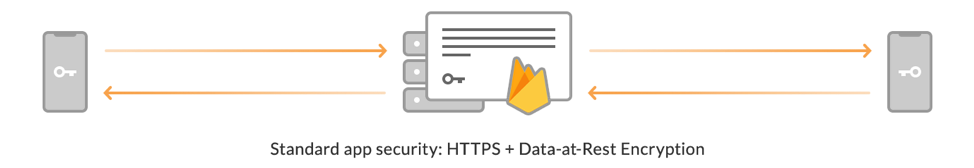
\includegraphics[width=15cm]{Backend_Implementierung/images/firebase_without_p2p_encryption.png}
		\caption{}
		\label{fig:firebase_without_encryption}
	\end{subfigure}\\
	\begin{subfigure}{\textwidth}
		\centering
		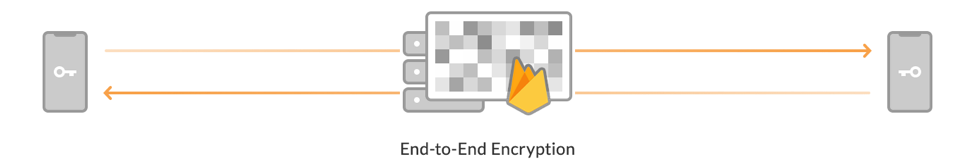
\includegraphics[width=15cm]{Backend_Implementierung/images/firebase_with_p2p_encryption.png}
		\caption{}
		\label{fig:firebase_with_encryption}
	\end{subfigure}
	\caption[]{ Firebase (a) ohne / (b) mit Ende-zu-Ende Verschlüsselung \protect \footnotemark}
\end{figure}
\footnotetext{Quelle: \url{https://virgilsecurity.com/blog/e3kit-for-firebase}, letzter Zugriff: 10. Mai 2021}

